\documentclass[a4paper, 12pt]{article}
\usepackage[OT1]{fontenc}
\usepackage{ngerman}
\usepackage[latin1]{inputenc}
\usepackage{graphics}
\usepackage{fancyhdr}
\usepackage{epsfig}
% nur f�r linux's pdflatex
%\usepackage{pdfpages}
%active table of contents but without borders
\usepackage[colorlinks=false,citebordercolor=111,menubordercolor=111,linkbordercolor=111]{hyperref}

\begin{document}

% Kopfzeile mit Kapitel
\renewcommand{\sectionmark}[1]{\markleft{#1}{}}
\pagestyle{fancyplain}
\rhead{\footnotesize\thepage}
\lhead{\footnotesize\leftmark}
\cfoot{}

%Titelseite
\begin{titlepage}
\title{
\includegraphics[width=7cm]{uniol.png}\\ \vspace{2cm}				
			\textbf{Palladio Componentmodel\\}
			{ \large Entwurfsbeschreibung\vspace{2cm}}}
			
			\author{Marko Hoyer\\ \textit{Marko.Hoyer@informatik.uni-oldenburg.de}}
\maketitle

\vspace{3cm}

\thispagestyle{empty}
\end{titlepage}

%Inhaltsverzeichnis
\tableofcontents
\thispagestyle{empty}
\newpage

%Einleitung
\section{Einleitung}
\label{sec:einleitung}

\subsection{Motivationen und Hintergr�nde}
\label{sec:einleitung:motivation}
Soll ein neu zu erstellendes Softwaresystem auf Basis vorhandener Komponenten erstellt werden, so stellt sich h�ufig die Frage nach der Performance des Gesamtsystems. Deren Beantwortung vor der Implementierung ist h�ufig Voraussetzung zur Einhaltung einiger nichtfunktionaler Anforderungen wie zum Beispiel der mittleren Antwortzeit. Werden die Antwortzeiten der Dienste der einzelnen Komponenten als bekannt vorausgesetzt, so gilt es nun, die Antwortzeit des Gesamtsystems mit einer bestimmten Konfiguration dieser Komponenten und ggf. Konnektoren zu ermitteln. Weiterhin ist h�ufig die Aufdeckung von 'Flaschenh�lsen' im System hilfreich, um durch eine gezielt andere Konfiguration der Komponenten die Performance zu erh�hen.
\par
Besteht das System ausschlie�lich aus linear zusammenh�ngenden Komponenten, deren Dienste der Reihe nach von einer ankommenden Anfrage durchlaufen werden, so gestaltet sich die Analyse des Systems recht einfach. Problemf�lle lassen sich anhand der Einzelzeiten identifizieren, und die gesamte Antwortzeit kann durch Addition der Einzelzeiten relativ leicht ermittelt werden.\\
Beinhalteten die Komponenten innerhalb des Systems jedoch Verzweigungen, so m�ssen alle sich ergebenen Pfade einzeln berechnet und mit einer bestimmten Gewichtung gewertet werden.\\
Weiterhin ergibt es sich in Systemen h�ufig, dass bestimmte Dienste einer Komponente von mehreren Diensten des Gesamtsystems ben�tigt werden. Ein Beispiel hierf�r sind Dienste, die Daten aus einer Datenbank auslesen. Hierbei geht die Analyse des Systems �ber die Pfade hinaus. Es m�ssen nun die Antwortzeiten der Dienste der Komponenten dynamisch auf die Anzahl zu einem Zeitpunkt ankommender Anfragen angepasst werden.\\
�bersteigt die mathematisch exakte Analyse des Systems bereits hier die Grenzen des sinnvoll machbaren, so erscheint die exakte Berechnung bei der Verteilung der einzelnen Komponenten auf verschiedene Prozessoren noch komplexer.
\par
An dieser Stelle kann die Simulation ansetzen. Es werden nun nicht mehr die mathematisch exakten Gegebenheiten berechnet, sondern anhand der Simulation eines Modells mit einer bestimmten Ungenauigkeit ermittelt. Weiterhin lassen sich bei der Simulation 'Flaschenh�lse' identifizieren, die bei der mathematischen Berechnung nur schwer zu ermitteln sind. Hierzu kann beispielsweise einfach das Zeitverhalten einer Anfrage Dienst f�r Dienst aufgezeichnet und hinterher ausgewertet werden. Bild \ref{pic:simul} zeigt schematisch eine solche Simulation.

\begin{figure}[ht]
\begin{center}
\fbox{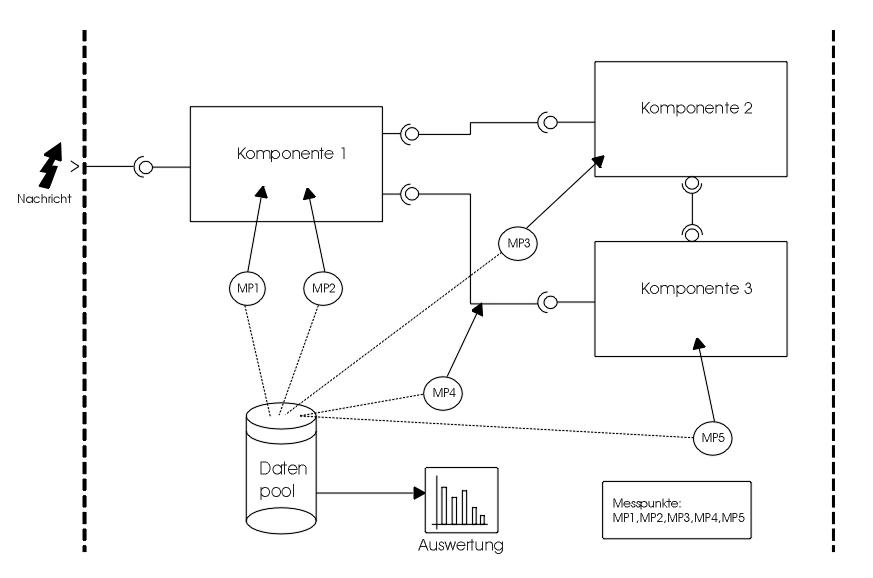
\includegraphics[width=13cm]{../res/simul.jpg}}
\caption{Schematische Darstellung der Simulation}
\label{pic:simul}
\end{center}
\end{figure}

\subsection{Ziele des Individuellen Projektes}
\label{sec:einleitung:ziele}
Ziel dieses Projektes ist die Erstellung einer Infrastruktur f�r die in Abschnitt \ref{sec:einleitung:motivation} erl�uterte Simulation in Form eines Frameworks. Bestandteil des Frameworks wird die Modellierung des Systems und der Komponenten, ein Modell zur Simulation von Anfragen an Dienste des Systems und die Auswertung der gesammelten Daten sein. Diese Bestandteile werden in einer Simulationsumgebung gekapselt.
\par
Bei der Entwicklung wird verst�rkt darauf geachtet, dass kleinere �nderungen und Erweiterungen des Frameworks nicht gro�e �nderungen der Implementierung zur Folge haben. So ist es beispielsweise w�nschenswert, dass einige sich von Modell zu Modell h�ufig �ndernde Bestandteile austauschen lassen, ohne eine Zeile Quellcode des Frameworks �ndern zu m�ssen. Weiterhin sollen Entwurfsentscheidungen, die die Umsetzung einer neuen Modellierung verhindern, �nderbar sein. Das bedeutet, dass die Bestandteile des Frameworks unabh�ngig voneinander austauschbar sein m�ssen.
\par
Das Projekt gliedert sich in die drei im Proposal \cite{lit:proposal} angegebenen Entwicklungsinkremente. Am Ende jedes Inkrementes wird ein der Entwicklungsstufe angepasster Prototyp entstehen, welcher das Framework in seinem aktuellen Stand benutzt.

\subsection{Aufbau dieser Ausarbeitung}
\label{sec:einleitung:aufbau}

Die Ausarbeitung gliedert sich in drei inhaltliche Teile, welche von dieser Einleitung und einem abschlie�enden Fazit eingeschlossen sind.
\par
Der erste Teil befasst sich mit der Kl�rung theoretischer Fragen in Bezug auf die Modellierung von Komponentenarchitekturen und der Simulation. Hierzu werden anf�nglich einige Grundlagen zur Modellierung von Komponenten erarbeitet, welche als Ziel das Modell der gesamten Komponentenarchitektur haben. Darauf aufbauend werden in diesem Modell potentielle Zeitverbraucher identifiziert. Der letzte Teil dieses Kapitels stellt das f�r das Framework entwickelte Simulationsmodell vor.
\par
Der zweite und gleichzeitig gr��te Teil dieser Ausarbeitung ist dem Entwurf des Frameworks gewidmet. Dieser beginnt mit dem Festlegen einiger allgemeiner Anforderungen an das Framework. Der zweite Teil dieses Kapitels erarbeitet eine sinnvolle Architektur des Frameworks. Das bedeutet, dass an dieser Stelle das Framework in seine groben Bestandteile gegliedert wird. Innerhalb dieser Teile werden dann unter Betrachtung von speziellen an den jeweiligen Teil gestellten Anforderungen einzelne Komponenten identifiziert. Der dritte Teil des Entwurfs bildet dann schlie�lich die Architektur mit ihren Komponenten auf Klassen und Pakete ab. Hier werden einige der Entwurfsentscheidungen zum besseren Verst�ndnis des Frameworks detailiert erkl�rt.
\par
Das dritte und abschlie�ende inhaltliche Kapitel der Ausarbeitung geht auf die Anwendung des Frameworks ein. Hierzu wird anhand eines Beispiels die Benutzung der Basisfunktionalit�t beschrieben. Weiterhin wird auf die Erweiterungsm�glichkeiten und deren Ansatzpunkte im Framework eingegangen. Um den Umfang der Funktionalit�t des Frameworks einsch�tzen zu k�nnen, wird dem Leser abschlie�end ein �berblick �ber die Grenzen des Frameworks vermittelt.

%Architektur
\section{Architektur}

In diesem Kapitel wird die derzeitige Architektur des Komponentenmodells vorgestellt. Sie setzt sich aus den in Abbildung \ref{fig:arch} dargestellten und im Folgenden kurz erl�uterten Bestandteilen zusammen. An der Umrandung der Bl�cke ist abzulesen, ob diese bereits entworfen oder lediglich als Erweiterungen geplant sind. Details und Informationen zur Umsetzung der Bestandteile des Komponentenmodells sind Inhalt der folgenden Kapitel dieses Dokuments.

\begin{figure}[ht]
 \centering 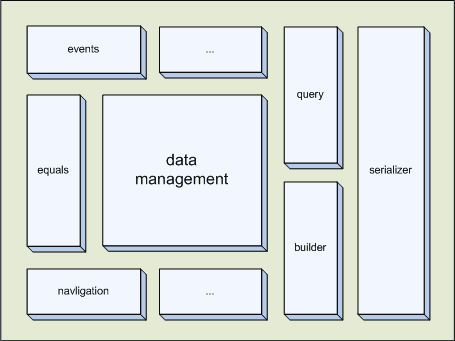
\includegraphics{arch.png}
 \caption{Architektur des Komponentenmodells}
 \label{fig:arch}
\end{figure}

Zentrum der Architektur bildet die in der Abbildung mit \emph{data management} bezeichnete Datenhaltung. Sie dient der lokalen Speicherung der Entit�ten und Relationen des Modells zur Laufzeit der nutzenden Anwendung. Hierf�r stellt sie M�glichkeiten zum Lesen und Schreiben der Daten zur Verf�gung. Die Konsistenz der Daten ist in dieser Schicht lediglich in Bezug auf die verwendeten Datenstrukturen zu gew�hrleisten. Semantische Fehler im Sinne des theoretischen Komponentenmodells sind von der Datenhaltung zu tollerieren, um unabh�ngig von m�glichen �nderungen dieser Semantik zu bleiben. Aufgrund dessen ist der das Modell nutzenden Anwendung keine M�glichkeit zu gew�hren, direkt auf die Datenhaltung zuzugreifen, da sonst Korrektheit im Sinne des theoretischen Modells nicht mehr gew�hrleistet werden kann. Zugriff ist erst nach �berpr�fung durch entsprechende Zwischenschichten zu gestatten.

Schreibende �nderungen der Anwendung am Modell sind hierbei durch den in der Architekur mit \emph{builder} bezeichneten Block vorgesehen. Dieser stellt eine Infrastruktur bereit, welche �nderungen an verschiedenen Stellen des Modells zul�sst und den korrekten Aufbau gem�� dem theoretischen Modell sicherstellt. Es k�nnen an dieser Stelle bereits durch geschickte Wahl der Zugriffsmethoden Fehler ausgeschlossen werden. Eine M�glichkeit der Umsetzung dieser Schicht unter Beachtung der Hierarchie des Komponentmodells wird in Kapitel \ref{sec:builder} vorgestellt.
  
Der lesende Zugriff auf das Modell kann je nach Bedarf durch verschiedene Schichten erfolgen. Die in Abbildung \ref{fig:arch} mit \emph{query} bezeichnete Schicht dient der Abfrage von Attributen der Entit�ten und der Beziehungen zwischen diesen. Eine direkte Abfragem�glichkeit der Datenhaltung ist prinzipiell m�glich, jedoch aufgrund fehlenden Wissens �ber das theoretische Modell unpraktikabel. Abstraktionen in diesem Sinn sind also ebenfalls Aufgabe der Abfrageschicht.

Die persistente Speicherung des Modells ist Aufgabe der Serialisierungsschicht. Diese soll nach M�glichkeit unabh�ngig von der genauen Art der Speicherung bleiben. Sowohl der Ex- und Import von Xml-Dateien, wie auch die Speicherung in einer relationalen Datenbank sollen m�glich sein. Ebenfalls ist die bin�re Speicherung in einem eigenen Datenformat denkbar. Eine Entkopplung vom Kern des Komponentenmodells durch austauschbare Module bietet hierbei die gr��te Flexibelit�t.
Der Zugriff der Serialisierungsschicht auf die lokal gehaltenen Daten kann auf zwei unterschiedliche Arten realisiert werden, direkter Zugriff auf den Kern oder indirekter Zugriff �ber die Abstraktionsschichten \emph{query} und \emph{builder}. Vorteil der ersten Variante ist die freie Wahl der Zugriffsmethoden auf die Daten. Je nach Art der Speicherung k�nnen Anfragen gezielt angepasst werden, um effizient schreiben oder lesen zu k�nnen. Nachteil hierbei ist jedoch die Pr�fung der Konsistenz und Korrektheit des Modells. Diese m�sste redundant zur \emph{builder}-Schicht implementiert werden. Weiterhin wird eine Abh�ngigkeit zwischen Kern und Serialisierungsschicht geschaffen, die im Falle der zweiten Variante nicht besteht. Die Nutzung der beiden Abstraktionschichten im zweiten Fall bilden weiterhin eine gute M�glichkeit zur effizienten Qualit�tssicherung. So schlagen Serialisierungstests fehl, wenn sich entweder Fehler in der Serialisierungsschicht selber oder in der Implementierung der Zugriffsmethoden befinden.

Der Benachrichtigung der nutzenden Software bei �nderungen des Modells dient die in der Abbildung mit \emph{events} bezeichnete Schicht. Ziel hierbei ist die Bereitstellung vollst�ndiger �berwachungsm�glichkeit des Modells ohne direkte Verbindung zu den Quellen der Ver�nderung. So sollen sowohl die �nderungen des Modells durch die Builder als auch durch die Deserialisierung �berwacht werden. Setzen sich zur Wahrung der Konsistenz und Korrektheit Aktionen transitiv fort, so sind auch diese �nderungen der �berwachung mitzuteilen.

Die in Abbildung \ref{fig:arch} mit \emph{navigation} und \emph{equals} bezeichneten Module sind als Erweiterungen geplant. Zweck des ersten Moduls ist die Navigation durch das Komponentenmodell z.B. entlang des Kontrollflusses unter Verwendung verschiedenster Strategien. Das zweite Modul befasst sich mit der �quivalenz von Bestandteilen eines Modells oder gar von gesamten Modellen. Die M�glichkeit der unterschiedlichen Definition von �quivalenz anhand verschiedener Kriterien ist hierbei wichtigste Anforderung an dieses Modul.

Die Architektur kann je nach Bedarf beliebig um Module und Schichten erweitert werden. Diese k�nnen entweder direkt oder indirekt �ber Abstraktionsschichten auf den Kern zugreifen. Bei direkten schreibenden Zugriffen ist wie oben bereits erl�utert zu beachten, dass die Konsistenz im Sinn des theoretischen Modells eingehalten werden muss. Keinesfalls d�rfen Erweitungsmodule der nutzenden Anwendung den direkten Zugriff auf den Kern erm�glichen. Ist direkter Zugriff nicht zwingend erforderlich, so sind die durch die entsprechenden Abstraktionsschichten angebotenen Schnittstellen vorzuziehen. 

In den folgenden Kapiteln werden die f�r die aktuelle Version des Komponentenmodells entworfenen Module und Schichten vorgestellt, Entwurfsentscheidungen begr�ndet und bekannte Probleme erl�utert.


%environment
\section{Instanzierung des Modells}

Das Komponentenmodell ist durch die im Namensraum \verb+Palladio.ComponentModel+ definierte Klasse \verb+ComponentModelEnvironment+ gekapselt. Diese l��t sich unter Verwendung des parameterlosen Konstruktors instanzieren. Mehrfache Instanzen des Komponentmodells sind problemlos m�glich, da auf die Verwendung von Klassen gem�� dem Singleton-Pattern basierend auf statischen Klassenvariablen \cite{lit:gof} verzichtet wurde. Beim Entwurf von Erweiterungen, die direkt in das Komponentenmodell einflie�en, ist dieses Konzept beizubehalten, um Kompatibelit�tsprobleme zu vermeiden. Konzepte zur Synchronisation zweier Modelle sind in der aktuellen Version des Komponentmodells nicht vorgesehen. Bestehen Anforderungen dieser Art, so sind diese unter Verwendung der Benachrichtigungsmechanismen in Verbindung mit der Anfrage und Builder-Schicht zu realieren.

Nach der Instanzierung steht ein leeres Modell zur Verf�gung. Wahlweise kann unter Verwendung der Builder (vgl. Kapitel \ref{sec:builder}) ein neues Modell erstellt oder ein persistent gespeichertes geladen werden. Alle Schnittstellen zu den jeweiligen Schichten sind �ber die das Modell kapselnde Klasse \verb+ComponentModelEnvironment+ erreichbar.

%Builder
\section{Aufbau eines neuen Modells}

%Events
\section{Benachrichtigung bei �nderungen im Modell}

%Query
\section{Suchanfragen an das Modell}

\subsection{Allgemeine Anfragen}

%Navigation
\subsection{Navigation im Modell}

%Equals
\subsection{Vergleichbarkeit zwischen Bestandteilen des Modells} 

%Serialisierung
\section{Persistente Speicherung des Modells}

%andere
\section{Erweiterungsm�glichkeiten}

%Literaturverzeichnis
\addcontentsline{toc}{section}{Literaturverzeichnis}%
\bibliographystyle{geralpha}
\bibliography{cm_entwurf}


\end{document}
